% !TeX encoding = UTF-8
% chktex-file 21 chktex-file -2 chktex-file 23
\documentclass[fontset=ubuntu,12pt,a4paper,fleqn]{article}
\usepackage[a4paper,left=1cm,right=1cm,top=1cm,bottom=1.5cm,bindingoffset=5mm]{geometry}
\usepackage[UTF8]{ctex}
\usepackage[utf8]{inputenc}
\usepackage[ngerman]{babel}
\usepackage{amsmath}
\usepackage{amsfonts}
\usepackage{amssymb}
\usepackage{commath}
\usepackage{helvet}
\usepackage[T1]{fontenc}
\usepackage{tikz}
\usepackage{pgfplots}
\usepackage{helvet}
\usepackage{tabu}
\usepackage{multicol}
\usepackage[pdftex,pdfa,hidelinks]{hyperref}
\usepackage[autostyle=true,german=quotes]{csquotes}

\setlength{\parindent}{0em} 
\pagenumbering{arabic}

\begin{document}

{\Large\textbf{Matrizenmultiplikation mit dem Falkschema}\par}

\setlength{\columnseprule}{0.4pt}
\begin{multicols}{2}

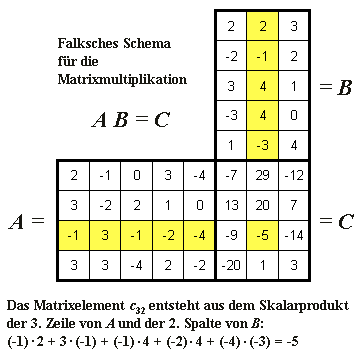
\includegraphics[width=0.7\linewidth]{FalkschesSchema.png}

{\Large\textbf{Einfache Ableitungsregeln}\par}

\textbf{Faktroregel:}
\[
y= C\cdot f(x) \Rightarrow y'= C\cdot f'(x)
\]
\textbf{Summenregel:}
\[
y= f_1(x) + f_2(x) + ... + f_n(x)  
\]\[
\Rightarrow y'=f'_1(x) + f_2'(x) + ... + f_n'(x)
\]
\textbf{Produktregel:}
\[
y= u(x) \cdot v(x) \Rightarrow y'=u'(x) \cdot v(x) + u(x) \cdot v'(x)
\]
\textbf{Quotientenregel:}
\[
y= \frac{u(x)}{v(x)} \Rightarrow y'=\frac{u'(x) \cdot v(x) - u(x) \cdot v'(x)}{[v(x)]^2}
\]
\textbf{Kettenregel:}
\[
y=a(b(c(x))) \Rightarrow y'= a'(x) \cdot b'(x) \cdot c'(x)
\]

\textbf{Wichtige Ableitungen:}
\begin{align*}
	f(x) &\Rightarrow f'(x)\\
	\ln(x) &\Rightarrow \frac{1}{x}\\
	\arccos(x) &\Rightarrow -\frac{1}{\sqrt{1-x^2}}\\
\end{align*}

\textbf{Wichtige Rechnungen:}
\begin{align*}
	\ln(1) &=0\\
	\sin^2(x)+\cos^2(x)&=1\\
	\sin\left(\frac{\pi}{2}\right) = \sin\left(\frac{3\pi}{2}\right) &=0\\
	\cos(0) = \cos(\pi) = \cos(2\pi)&=0\\
	\sin(0) = \sin(\pi) = \sin(2\pi)&=1\\
	\cos\left(\frac{\pi}{2}\right) = \cos\left(\frac{3\pi}{2}\right) &=1\\
\end{align*}

\textbf{Klausurtestaufgabe:} Gegeben seien die Funktionen f,g durch\\
{\fontsize{9}{10} \(g(x,y)=\begin{pmatrix}
x+y \\ x^2-y \\ 2xy
\end{pmatrix},\ f(x,y,z)=\begin{pmatrix}
\sin(x) \\ \sin(y+z)
\end{pmatrix}\)

Berechnen Sie die Jacobi-Matrix von \(f\circ g\) mit Hilfe der Kettenregel: \(D(f\circ g)(x,y)=Df(g(x,y))\cdot Dg(x,y)\).

\textbf{Hinweis}: Zur Berechnung von \(Df(g(x,y))\) berechnen Sie zunächst \(Df(x,y,z)\) und setzen Sie anschließend den Ergebnisvektor von \(g(x,y)\) ein.

\[Df(x,y,z)=\begin{pmatrix}
\cos(x) & 0 & 0 \\
0 & \cos(y+z) & \cos(y+z) \\\end{pmatrix}\]
\[Df(x+y,x^2-y,2xy)=\]
\[\begin{pmatrix}
\cos(x+y) & 0 & 0 \\
0 & \cos(x^2-y+2xy) & \cos(x^2-y+2xy) \\\end{pmatrix}\]
\[Dg(x,y)=\begin{pmatrix}
1 & 1 \\
2x & -1 \\
2y & 2x\end{pmatrix}\]
\[D(f\circ g)(x,y)=\begin{pmatrix}
\cos(x+y) & \cos(x+y) \\
2\cos\alpha(x+y) & \cos\alpha(2x-1) \\
\end{pmatrix}\]}
\newpage
\end{multicols}






{\Large\textbf{Partielle Ableitungen}\par}

\textbf{Bildung partieller Ableitungen:}
Die partiellen Ableitungen einer Funktion $f(x_1,x_2,x3)= x_1\cdot x_2+x3$ lassen sich sich wie folgt bestimmen:
\begin{align*}
\frac{\partial f}{\partial x_1}(x_1,x_2,x_3) &= 1\cdot x_2\\
\frac{\partial f}{\partial x_2}(x_1,x_2,x_3) &= x_1\cdot 1\\
\frac{\partial f}{\partial x_3}(x_1,x_2,x_3) &= 1
\end{align*}

\textbf{Berechnung der Tangentialebene:}
Es seien \(\mathbb{D} \subset \mathbb{R}^2, f:\mathbb{D}->\mathbb{R}\) eine partiell differenzierbare Funktion und \((x_{01},x_{02})\in\mathbb{D}\). Dann lautet die Gleichung der Tangentialebene für den Punkt \((x_{01},x_{02})\):

\begin{align*}
x_3&=f(x_{01},x_{02})+\dpd{f}{x_1}(x_{01},x_{02})(x_1-x_{01})+\dpd{f}{x_2}(x_{01},x_{02})(x_2-x_{02})\\
&=f(x_{01},x_{02})+\begin{pmatrix} \dpd{f}{x_1} (x_{01},x_{02}) & \dpd{f}{x_2}(x_{01},x_{02}) \end{pmatrix} \cdot \begin{pmatrix} (x_1-x_{01})\\ (x_2-x_{02}) \end{pmatrix}
\end{align*}

Zuerst den Punkt $(x_{01},x_{02})$ an den Stellen $x_{01}$ und $x_{02}$ einsetzen. Dann ausrechnen und am Ende den Punkt für  $x_{1}$ und $x_{2}$ einsetzen um zum Ergebnis für x3 an dem genannten Punkt zu kommen.\\

\textbf{Berechnung Gradient:}
Es sei \(\mathbb{D} \subset \mathbb{R}^n\) und \(f:\mathbb{D} \to \mathbb{R}\) partiell differenzierbar. Dann heißt der Vektor \(\mathrm{grad} f(x) = \begin{pmatrix}
\dpd{f}{x_1}(x) \\
\dpd{f}{x_2}(x) \\
\vdots \\
\dpd{f}{x_n}(x) \\
\end{pmatrix}\) der Gradient von \(f\) im Punkt \(x\in\mathbb{D}= (x_1,\dots,x_n)\).\\Anstelle von \(\mathrm{grad} f(x)\) wird auch häufig \(\nabla f(x)\) geschrieben.\\

\textbf{Partielle Ableitungen k-ter Ordnung:}

Es sei \(D\subset\mathbb{R}^n,f:D\to\mathbb{R}\) eine partiell differenzierbare Funktion und \(x_0 \in D\). Die Funktion f heißt \\ zweimal \textbf{partiell differenzierbar} in \(x_0\), wenn alle partiellen Ableitungen \(\pd{f}{x_i}\) in \(x_0\) wieder partiell differenzierbar sind.

Man schreibt \(\frac{\partial^2 f}{\partial x_j x_i}(x_0)=\pd{}{x_j}\left(\pd{f}{x_i}\right)(x_0)=f_{x_j x_i}(x_0)\)

Dieser Ausdruck heißt dann \textbf{zweite partielle Ableitung} von f.

Allgemein heißt f \textbf{k-mal partiell differenzierbar}, wennn alle (k-1)-ten partiellen Ableitungen von f wieder partiell differenzierbar sind. Man schreibt:

\[\dpd{f}{x_{ik} \partial x_{i(k-1)} \dots \partial x_{i1}}(x_0) = \frac{\partial}{\partial x_{ik}}\left(\frac{\partial^{k-1} f}{\partial x_{i(k-1)} \dots \partial x_{i1}}\right)(x_0)=f_{x_{ik} \dots x_{i1}}\]

\textbf{Satz von Schwarz:}
Es sei \(D\subset\mathbb{R}^n,f:D\to\mathbb{R}\) zweimal stetig partiell differenzierbar. Dann ist \(\frac{\partial^2 f}{\partial x_i \partial x_j}=\frac{\partial^2 f}{\partial x_j \partial x_i}\) für alle \(i,j\in\left\{1,\dots,n\right\}\). Die Reihenfolge der Ableitungsvariablen spielt also keine Rolle.
\newpage








{\Large\textbf{Totale Differenzierbarkeit}\par}
\textbf{Vektorfunktion:}
Eine eindeutige Abbildung \(f:\mathbb{D}\to W,\mathbb{D}\subset\mathbb{R}^n,W\subset\mathbb{R}^m,m>1\) mit mehrdimensionalem Wertebereich heißt \textbf{Vektorfunktion}.
     
\begin{multicols}{2}
\textbf{Beispiel:}
Es sei \(\mathbb{D}\subset\mathbb{R}^3\to\mathbb{R}^2\) gegeben durch
\[f(x_1,x_2,x_3)=\begin{pmatrix}
x_1+x_3 \\ x_2+x_3
\end{pmatrix}\]
$f(x_1,x_2,x_3)$ hat 2 Ergebniskomponenten:
\[f_1(x_1,x_2,x_3)=x_1+x_2\]
\[f_2(x_1,x_2,x_3)=x_2+x_3\]
\end{multicols}

\begin{multicols}{2}
\textbf{Jacobi-Matrix:}
Es sei \(f:\mathbb{D}\to \mathbb{R}^m,\mathbb{D}\subset\mathbb{R}^n\) eine Abbildung und \(x_0\in\mathbb{D}\). Weiterhin sei f in \(x_0\) total differenzierbar mit der Matrix
\[A=(a_{ij});i=1,\dots,m;j=1,\dots,n \in\mathbb{R}^{m\times n}\]
Dann ist f in \(x_0\) stetig und alle Komponentenfunktionen \(f_1,\dots,f_m:\mathbb{R}^n\to\mathbb{R}\) sind in \(x_0\) partiell differenzierbar, wobei gilt: \(a_{ij}=\pd{f_i}{x_j}(x_0)\).\\
Die Matrix heißt Funktionalmatrix oder auch Jacobi-Matrix von f und wird mit \(Df(x_0)\) oder \(J_f(x_0)\) bezeichnet.
\[Df(x_0)=\begin{pmatrix}
\dpd{f_1}{x_1}(x_0) & \dpd{f_1}{x_2}(x_0) & \cdots & \dpd{f_1}{x_n}(x_0) \\
\dpd{f_2}{x_1}(x_0) & \dpd{f_2}{x_2}(x_0) & \cdots & \dpd{f_2}{x_n}(x_0) \\
\vdots & \vdots & \ddots & \vdots \\
\dpd{f_m}{x_1}(x_0) & \dpd{f_m}{x_2}(x_0) & \cdots & \dpd{f_m}{x_n}(x_0)
\end{pmatrix}\]
\end{multicols}
\textbf{Totale Differenzierbarkeit:}
Sei \(f:\mathbb{R}^2\to\mathbb{R}\) eine total differenzierbare Funktion. Dann kann f in der Nähe eines Punktes \((x_{01},x_{02})\in\mathbb{R}^2\) durch \(f(x_{01},x_{02})+Df(x_{01},x_{02})\begin{pmatrix}x_1-x_{01} \\ x_2-x_{02}\end{pmatrix}\) angenähert werden.

Es gilt also \(f(x_1,x_2)=f(x_{01},x_{02})+\begin{pmatrix}
\dpd{f}{x_1}(x_{01},x_{02}) & \dpd{f}{x_2}(x_{01},x_{02})\end{pmatrix}\begin{pmatrix}
x_1-x_{01} \\ x_2-x_{02}
\end{pmatrix}\)

\[f(x_1,x_2)-f(x_{01},x_{02})\approx\dpd{f}{x_1}(x_{01},x_{02})\cdot\underbrace{(x_1-x_{01})}_{=:\Delta x_1} + \dpd{f}{x_2}(x_{01},x_{02})\cdot\underbrace{(x_2-x_{02})}_{=:\Delta x_2}\]

also gilt: \(\Delta f\approx \pd{f}{x_1}\cdot\Delta x_1 + \pd{f}{x_2}\cdot\Delta x_2\)

Für \enquote{beliebig kleines} \(\Delta x_1\) und \(\Delta x_2\) schreiben wir \enquote{d} statt \enquote{\(\Delta\)} und \enquote{=} statt \enquote{\(\approx\)}.

\[\boxed{df = \dpd{f}{x_1}(x_{01},x_{02})\cdot dx_1 + \dpd{f}{x_2}(x_{01},x_{02})\cdot dx_2} \]
Diesen Ausdruck bezeichnet man als \textbf{totales Differenzial} der Funktion f.

Für eine Funktion \(f:\mathbb{R}^n\to\mathbb{R}\) gilt:
\[\boxed{df = \dpd{f}{x_1}\cdot dx_1 + \dpd{f}{x_2}\cdot dx_2 + \cdots + \dpd{f}{x_2}\cdot dx_n}\]

\textbf{Berechnung linearer maximaler absoluter Fehler:} 
\[\left|\Delta f\right|\approx \left|\dpd{f}{x_1}(x_1,\dots,x_n)\right|\cdot\left|\Delta x_1\right|+\cdots+\left|\dpd{f}{x_n}(x_1,\dots,x_n)\right|\cdot\left|\Delta x_n\right|\]
\newpage







{\Large\textbf{Extremwerte}\par}

\textbf{Bestimmung lokales Extremum:} Es sei \(U \subset \mathbb{R}^n\) eine offene Menge und \(f:U\to\mathbb{R}\) differenzierbar. Besitzt f in \(x_0\in U\) ein lokales Extremum, so gilt:
\(\boxed{\nabla f(x_0)=0}\) d.h. \(\boxed{\pd{f}{x_1}(x_0)=\cdots=\pd{f}{x_n}(x_0)=0}\)\\

\textbf{Definitheit einer Matrix:} 
Eine Matrix \(A=(a_{ij}), i,j=1,\dots,n \in \mathbb{R}^{n\times n}\) heißt \textbf{positiv definit}, falls gilt:
{\fontsize{9}{10}
\begin{multicols}{2}
\(a_{11}>0,\det\begin{pmatrix}
a_{11} & a_{12} \\ a_{21} & a_{22}
\end{pmatrix} > 0, \dots, \det\begin{pmatrix}
a_{11} & \cdots & a_{1n} \\
a_{21} & \cdots & a_{2n} \\
\vdots & \ddots & \vdots \\
a_{n1} & \cdots & a_{nn}
\end{pmatrix} > 0\), 

also \(\det\begin{pmatrix}
a_{11} & \cdots & a_{1k} \\
a_{21} & \cdots & a_{2k} \\
\vdots & \ddots & \vdots \\
a_{k1} & \cdots & a_{kk}
\end{pmatrix} > 0\) für alle \(k=1,\dots,n\).

A heißt \textbf{negativ definit}, falls -A positiv definit ist.\\
\textbf{Berechnung der Determinante einer 2x2 Matrix:} \\

\(\det\begin{pmatrix}
a & b  \\ c & d
\end{pmatrix}
=  (a\cdot d) - (c\cdot b)\)
\\\\
\textbf{Berechnung der Determinante einer 3x3 Matrix:} 
\begin{align*}
\det\begin{pmatrix}
a & b & c  \\ d & e & f \\ g & h & i
\end{pmatrix}=&(a \cdot e \cdot i) + (b \cdot f \cdot g) + (c \cdot d \cdot h)\\
& - (g \cdot e \cdot c) - (h \cdot f \cdot a) - (i \cdot d \cdot b)
\end{align*}
\end{multicols}
}
\textbf{Hesse Matrix:}
Es seien \(U\subset\mathbb{R}^n\) eine offene Menge, \(f:U\to\mathbb{R}\) eine zweimal stetig partiell differenzierbare Funktion und \(x_0\in U\). Unter der \textbf{Hesse-Matrix} von f in \(x_0\) versteht man die Matrix: \[H_f(x_0)=\begin{pmatrix}
\frac{\partial^2 f}{\partial x_1^2}(x_0) & \cdots & \frac{\partial^2 f}{\partial x_1 \partial x_n}(x_0) \\
\frac{\partial^2 f}{\partial x_2 \partial x_1}(x_0) & \cdots & \frac{\partial^2 f}{\partial x_2 \partial x_n}(x_0) \\
\vdots & \ddots & \vdots \\
\frac{\partial^2 f}{\partial x_n \partial x_1}(x_0) & \cdots & \frac{\partial^2 f}{\partial x_n^2}(x_0) \\
\end{pmatrix}\]

\textbf{Aussagen über Extremstellen:}
Es sei \(U\subset\mathbb{R}^n\) eine offene Menge, \(f:U\to\mathbb{R}\) zweimal stetig differenzierbar und \(x_0\in U\) ein Punkt mit \(\nabla f(x_0)=0\).
\begin{enumerate}
	\item Ist \(H_f(x_0)\) positiv definit, so hat f in \(x_0\) ein lokales Minimum.
	\item Ist \(H_f(x_0)\) negativ definit, so hat f in \(x_0\) ein lokales Maximum.
	\item Ist \(textbf{U\subset\mathbb{R}^2}\) und gilt \(\det H_f(x_0) < 0\), so liegt kein Extremwert vor.
\end{enumerate}

\textbf{Beispiel:}
Gegeben sei die Funktion \(f:\mathbb{R}^2\to\mathbb{R}\) durch \(f(x_1,x_2)=\cos(x_1)+\cos(x_2)\)

Gradient: \(\nabla f(x_1,x_2)=\begin{pmatrix}
-\sin x_1 \\ -\sin x_2
\end{pmatrix} := \begin{pmatrix}
0 \\ 0
\end{pmatrix} \to -\sin x_1 = -\sin x_2 = 0\)

\((k_1\pi,k_2\pi), k_1,k_2\in\mathbb{Z}\)
{\fontsize{9}{10}\begin{multicols}{2}
Hesse-Matrix

\(H_f(x_1,x_2)=\begin{pmatrix}
-\cos x_1 & 0 \\ 0 & -\cos x_2
\end{pmatrix}\)

\(H_f(k_1\pi,k_2\pi)=\begin{pmatrix}
-{(-1)}^{k_1} & 0 \\ 0 & -{(-1)}^{k_2} 
\end{pmatrix}\)

\vspace{1cm}
\def\arraystretch{1.25}	
\begin{tabular}{ c | c | c }
	& \(k_1\) gerade & \(k_1\) ungerade \\ \hline
	\(k_2\) gerade & lokales Maximum & kein Extremwert \\ \hline
	\(k_2\) ungerade & kein Extremwert & lokales Minimum \\ 
\end{tabular}
\end{multicols}}
\newpage








{\Large\textbf{Integralrechnung}\par}
\begin{multicols}{2}
\textbf{Grundlegendes zu Mehrfachintegralen:} Es sei \(U\subset\mathbb{R}^2\) eine beschränkte und konvexe Menge und \(f:U\to\mathbb{R}\) eine stetige Funktion. Da U beschränkt ist, gibt es einen kleinsten vorkommenden x-Wert a und einen größten vorkommenden x-Wert b.

Der Flächeninhalt der Schnittfläche des Körpers bei einem beliebigen x-Wert zwischen a und b wird mit \(I(x)\) bezeichnet.

Der Körper, dessen Volumen wir ausrechnen, setzt sich aus all diesen Schnittflächen zusammen. Für jedes \(x\in [a,b]\) existiert eine Schnittfläche mit Flächeninhalt \(I(x)\), das heißt durch Aufsummieren dieser unendlich vielen Flächeninhalte ergibt sich das Volumen des Körpers.

\[\iint_U f(x,y)dxdy = \int^a_b I(x)dx\]

Der Flächeninhalt von \(I(x)\) kann einfach mit einem eindimensionalen Integral berechnet werden.

\[I(x) = \int^{y_o(x)}_{y_u(x)} f(x,y)dy \]

Insgesamt ergibt sich also:

\[\iint_U f(x,y)dxdy = \int^b_a \left(\int^{y_o(x)}_{y_u(x)} f(x,y)dy\right)dx\]
\end{multicols}

\textbf{Beispiel:} \(U=\{(x,y):0 \leq x \leq 1, x^2 \leq y \leq \sqrt{x}\}\)

\begin{tikzpicture}
\begin{axis}
[
xlabel=x,
ylabel=y,
xmin=0,
ymin=0,
ymax=1,
xmax=1,
width=5cm,
]
\addplot[domain=0:1,mark=none,samples=200] {x^2};
\addplot[domain=0:1,mark=none,samples=200] {sqrt(x)};
\end{axis}
\end{tikzpicture}


\(\iint_U f(x,y)dxdy=\int_0^1 \left(\int_{x^2}^{\sqrt{x}} (x^2+y) dy\right)dx = \frac{33}{140}\)
\\\\
\textbf{Ebenso im Dreidimensionalen: }
Es seien \(U\subset\mathbb{R}^3\) eine beschränkte und konvexe Menge und \(f:U\to\mathbb{R}\) eine stetige Funktion. Weiterhin sei a der in U kleinste vorkommende x-Wert und b der größte.

Für \(x\in[a;b]\) bezeichnen wir den kleinsten y-Wert, für den es ein z gibt, sodass \((x,y,z)\in U\) gilt, mit \(y_u(x)\), und den größten mit \(y_o(x)\).

Schließlich bezeichnen wir für zulässiges (x,y) mit \(z_u(x,y)\) den kleinsten z-Wert, sodass \((x,y,z)\in U\), und mit \(z_o(x,y)\) den größten z-Wert. Dann ist \[\iiint_U f(x,y,z)dxdydz=\int_a^b \left(\int_{y_u(x)}^{y_o(x)} \left(\int_{z_u(x,y)}^{z_o(x,y)} f(x,y,z)dz\right)dy\right)dx\]

\textbf{Beispiel:}
\begin{multicols}{2}
	\begin{enumerate}
		\item \(U=[-1;1]\times[0,1]\times[0,2]\)
		
		\(f(x,y,z)=x^2+y^2+z^2\)
		
		\(int_{-1}^1 \left(\int_0^1 \left(\int_0^2 x^2+y^2+z^2dz \right)dy \right)dx\)
		
		\item \(U=\{(x,y,z):x,y,z \ge 0,x \le 1,y \le x,z \le y\}\)
		
		\(f(x,y,z)=x\cdot y^2 \cdot z\)
	\end{enumerate}
\end{multicols}
 


\newpage















{\Large\textbf{Differentialgleichungen}\par}
\textbf{Trennung der Variablen:} 
Gegeben sei die Gleichung \(y'=xy\).
Gesucht ist die Funktion \(y(x)\).

\(y'=\frac{dy}{dx} \to \frac{dx}{dy}=xy \to_{y \ne 0} \frac{dy}{y}=xdx\)\\

\begin{multicols}{2}
	\textbf{Wronski-Determinante:} Es sei \(L_H\) die Lösungsmenge einer linearen homogenen Differentialgleichung n-ter Ordnung. Dann gibt es n linear unabhängige Lösungen \(y_1,\dots,y_n\) der Differentialgleichung und es gilt: \(L_H=\{c_1y_1(x)+\cdots+c_n y_n(x)\}|c_1,\dots,c_n\in\mathbb{R}\).
	
	Aus den Grundlösungen \(y_1,\dots,y_n\) lässt sich also mit Hilfe von Linearkombinationen die gesamte Lösungsmenge berechnen.
	
	Weiterhin sind n Lösungen \(y_1,y_n \in L_H\) genau dann linear unabhängig, wenn für die \textbf{Wronski- Determinante} folgendes gilt:
	\[W(x)=\det\begin{pmatrix}
	y_1(x) & \cdots & y_n(x) \\
	y_1'(x) & \cdots & y_n'(x) \\
	\vdots & \ddots & \vdots \\
	y_1^{(n-1)}(x) & \cdots & y_n^{(n-1)}(x)
	\end{pmatrix} \ne 0 \]
	Dabei genügt schon \(W(x) \ne 0\) für ein x.


\textbf{Lineare Differentialgleichungen mit konstanten Koeffizienten:}
Für die Gleichung
\[y^{(n)}(x) + a_{n-1} \cdot y^{(n-1)}(x) + \cdots + a_1 \cdot y'(x) + a_0 \cdot y(x) = 0\]
wird ein Ansatz verwendet, der eine e-Funktion enthält.

\textbf{Ansatz:} \(y(x)=e^{\lambda x},\lambda\in\mathbb{R}\)

Differenzieren und Einsetzen des Ansatzes führt zu: \\ \(e^{\lambda x}\underbrace{(\lambda^n+a_{n-1}\lambda^{n-1}+\cdots+a_1\lambda+a_0)}=0\)

wird 0, falls \(\lambda\) eine Nullstelle des Polynoms \(P(x)=x^n+a_{n-1}x^{n-1}+\cdots+a_1x+a_0\) ist.\\

\textbf{Charakteristisches Polynom:}
Es sei \(y^{(n)}(x) + a_{n-1} \cdot y^{(n-1)}(x) + \cdots + a_1 \cdot y'(x) + a_0 \cdot y(x) = 0\) eine homogene lineare Differentialgleichung mit konstanten Koeffizienten.

Dann heißt das Polynom \(P(x)=x^n+a_{n-1}x^{n-1}+\cdots+a_1x+a_0\) \\ \textbf{charakteristisches Polynom der Differentialgleichung}.\\

Es sei \(y^{(n)}(x) + a_{n-1} y^{(n-1)}(x) + \cdots + a_1 y'(x) + a_0 y(x) = 0\) eine homogene lineare Differentialgleichung mit konstanten Koeffizienten. Ihr charakteristisches Polynom \(P(x)\) habe k reelle Nullstellen \(\lambda_1,\dots,\lambda_k\) mit \(P(x)={(x-\lambda_1)}^{m_1}{(x-\lambda_2)}^{m_2} \dots {(x-\lambda_k)}^{m_k}\), d.h. \(\lambda_j\) ist \(m_j\)-fache Nullstelle von P. Dann bilden die Funktionen
\begin{align*}
e^{\lambda_1 x},x \cdot e^{\lambda_1 x},\dots,x^{m_1-1} \cdot e^{\lambda_1 x} \\
e^{\lambda_2 x},x \cdot e^{\lambda_2 x},\dots,x^{m_2-1} \cdot e^{\lambda_2 x} \\
\vdots \hspace{1cm} \vdots \hspace{1cm} \\
e^{\lambda_k x},x \cdot e^{\lambda_k x},\dots,x^{m_k-1} \cdot e^{\lambda_k x}
\end{align*}
ein Fundamentalsystem der Differentialgleichung.
\textbf{Inhomogene Differentialgleichung:}
Liegt eine inhomogene Differentialgleichung mit Störfunktion \(b(x)\) vor, so kann in einigen Fällen eine geeignete Ansatzfunktion zur Lösung der Differentialgleichung verwendet werden:

Liegt zum Beispiel die Störfunktion in der folgenden Form vor

\(b(x)=a_n x^n + a_{n-1} x^{n-1} + \cdots + a_1 x + a_0\), so kann die folgende Ansatzfunktion verwendet werden:

\(\alpha_n x^n + \alpha_{n-1} x^{n-1} + \cdots + \alpha_1 x + \alpha_0\)
\end{multicols}
\newpage














\textbf{Beispiel:}
Zu lösen ist \(y'''-3y'-2y=4x^2\)

Zunächst homogene Differentialgleichung betrachten: \(y'''-3y'-2y=0,P(x)=x^3-3x-2\)

\(\lambda_1=-1,\lambda_2=2,\lambda_3=-1\)

Lösung der homogenen Differentialgleichung: \(y(x)=c_1xe^{-x}+c_2e^{-x}+c_3e^{2x}\)

Ansatz für die Störfunktion: Da \(b(x)=x^2\) ein Polynom 2. Grades ist, wird der Ansatz \(\underbrace{\alpha_2x^2+\alpha_1x+\alpha_0}_{y_P}\) verwendet.

\({y_P}'''=0,{y_P}''=2\alpha_2,{y_P}'=2\alpha_2x+\alpha_1\)

\(-6\alpha_2x-3\alpha_1-2\alpha_2x^2-\alpha_1x-2\alpha_0=4x^2\)

\(x^2\underbrace{(-2\alpha_2)}_4+x\underbrace{(-6\alpha_2-\alpha_1)}_0+\underbrace{(-3\alpha_1-2\alpha_0)}_0=4x^2+0x+0\)

\(\alpha_2=-2,\alpha_1=6,\alpha_0=-9\)

Lösung der inhomogenen Differentialgleichung: \(y(x)=c_1xe^{-x}+c_2e^{-x}+c_3e^{2x}-2x^2+6x-9,\ x\in\mathbb{R},c_i\in\mathbb{R}\)

\newpage












{\Large\textbf{Differentialgleichungssysteme (DGLS)}\par}
\textbf{Definition:} Ein System von m Gleichungen, dass die unbekannten Funktionen \(y_1(x),y_2(x),\dots,y_m(x)\) sowie deren Ableitungen \\
\({y_1}'(x),{y_1}''(x),\dots,{y_1}^{(n_1)}(x),\dots,{y_m}'(x),{y_m}''(x),\dots,{y_m}^{(n_m)}(x)\) enthält, heißt \\ \textbf{Differentialgleichungssystem}.
\begin{multicols}{2}
	\textbf{Beispiel:}
	Zu lösen ist das Differentialgleichungssystem
	\begin{align*}
	{y_1}' &= -2y_1+8y_2\ (*) \\
	{y_2}' &= -4y_1+6y_2+10x^2+16x-8\ (**) \\
	\end{align*}
	Eliminationsmethode:
	
	\((*)\) ableiten: \({y_1}'' = -2{y_1}'+8{y_2}'\)
	
	\((**)\) einsetzen: \({y_1}'' = -2{y_1}'-32y_1+48y_2+80x^2+128x-64\) \\
	\( y_1'=-2y_1+8y_2 (*) \) \\
	\(y_2')-4y_1+6y_2+10x^2+16x-8 (**) \) \\
	\( y_1''=-2y_1+8(-4y_1+6y_2+10x^2+16x-8) \) \\
	\( =-2y_1'-32y_1+48y_2+80x^2+128x-64  \overline{(*)}' \) \\
	\( (*) \) umstellen nach \( y_2 \) \\ 
	\( y_2=\frac{1}{8}y_1'+\frac{1}{4}y_1 \) \\
	Einsetzen in \( \overline{(*)}' \) \\
	\( \rightarrow y_1''=-2y_1'=-32y_1+48(\frac{1}{8}y_1'+\frac{1}{4}y_1) + 80x^2+128x-64 \) \\
	\(y_1'(-2+6)+y_1(-32+12)+89x^2+128x-64 \) \\
	\(\rightarrow y_1'''-4y_1'+20y_1=80x^2+128x-64 (***) \) \\
	\(\rightarrow \) homogene DGL \(\rightarrow \) charakteristisches Polynom: \(P(x)=x^2-4x+20 \) \\
	\(a=0; b=-4;c=20\) \\
	\(\lambda_{1,2}=2\pm4i \) \\
	\(y_1=\cos(4x)\cdot e^{2x} \) \\
	\(y_2=\sin(4x)\cdot e^{2x} \) (Eulersche Form)\\
	\(e^{\lambda x}=e^{(2+4i)x}=e^{2x}(\cos(4x)+i\sin(4x)) \) \\
	Ansatz für die inhomogene Lösung: \\
	\(y_p=\alpha_2x^2+\alpha_1x+\alpha_0 \) \\
	\(y_p'=2\alpha_2x+\alpha_1, y_p''=2\alpha_2, y_p'''(x)=0 \) \\
	Einsetzen in (***) für \(y_1, y_1', y_1''\) \\
	\( 2\alpha_2-4(2\alpha_2x+\alpha_1)+20(\alpha_2x^2+\alpha_1x+\alpha_0) = 80x^2+128x-64 \) \\
	Sortieren: \(x^2(20\alpha_2)+x(-8\alpha_2+20\alpha_1)+(2\alpha_2-4\alpha_1+20\alpha_0)\)
	\\ Koeffizientenvergleich \(20\alpha_2 = 80 \) usw. \\
	\(\alpha_0=-2 \)\\
	\(\alpha_1=8 \)\\
	\(\alpha_2=4 \)\\
	\( y_1(x)=\underbrace{c_1\cdot\cos(4x)e^{2x}+c_2\cdot\sin(4x)e^{2x}}_{\text{Homogone LSG}}+\underbrace{4x^2+8x-2}_{\text{Partikuläre LSG}}\)  (****) \\ \(x\in\mathbb{R}\) \\ \(c_1,c_2\in\mathbb{R}\) \\
	\(y_2=\frac{1}{8}y_1'+\frac{1}{4}y_1\)\\
	\(y_1'(x)=-4c_1\cdot\sin(4x)e^{2x}+2c_1\cdot\cos(4x)e^{2x}+4c_2\cdot\cos(4x)e^{2x}+2c_2\cdot\sin(4x)e^{2x}+8x+8 \) \\
	\(=e^{2x}\cdot\cos(4x)(
	\frac{1}{2}c_1+\frac{1}{2}c_2
	)+e^{2x}\cdot\sin(4x)(
	-\frac{1}{2}c_1+\frac{1}{2}c_2
	)+x^2+3x+\frac{1}{2} \) \\
	Vektorschreibweise: \\
	\(c_1=2D_1\) \\
	\(c_2=2D_2\) \\
	\( \vec{y}(x)=\begin{pmatrix}
	y_1(x) \\ y_2(x)
	\end{pmatrix}=\begin{pmatrix}2D_1 \\ D_1+D_2 \end{pmatrix} e^{2x}\cdot\cos(4x)+\begin{pmatrix}2D_2 \\ -D_1+D_2 \end{pmatrix}e^{2x}\cdot\sin(4x) + \begin{pmatrix}4x^2+8x-2 \\ x^2+3x +\frac{1}{2} \end{pmatrix} \)\\\(x\in\mathbb{R} D_i\in\mathbb{R}\)
\end{multicols}







\end{document}  